\PassOptionsToPackage{table}{xcolor}
\documentclass{article}
\usepackage[utf8]{inputenc}
\usepackage{xspace}
\usepackage{url}
\usepackage{hyperref}
\usepackage{fancyhdr}
\usepackage{cite}
\usepackage{pgfgantt}
\usepackage{todonotes}
\usepackage[icelandic,UKenglish]{babel}
\usepackage[UKenglish]{datetime}
\usepackage[T1]{fontenc}
\usepackage{graphicx}
\usepackage[table]{xcolor}
\usepackage{enumitem}% http://ctan.org/pkg/enumitem
\usepackage[gen]{eurosym}
\usepackage{multicol}
\graphicspath{ {./images/} }
\usepackage[titletoc,title]{appendix}
\usepackage{pdfpages}

\fancypagestyle{plain}{ %
  \fancyhf{} % remove everything
  \renewcommand{\headrulewidth}{0pt} % remove lines as well
  \renewcommand{\footrulewidth}{0pt}
}
% \setlength{\topskip}{0mm}
\setlength{\headheight}{15pt}
% \setlength{\topmargin}{-5.4mm}
% \setlength{\textheight}{230mm}
\setlength{\textwidth}{180mm}
\setlength{\oddsidemargin}{-5.0mm}
% \setlength{\evensidemargin}{10.0mm}
% \setlength{\captionmargin}{7mm}

\newenvironment{MYitemize}{%
    %% \renewcommand{\labelitemi}{$\rightarrow$}%
    %% \renewcommand{\labelitemii}{$\circ$}%
    %% \renewcommand{\labelitemii}{$\rightarrow$}%
    %% \renewcommand{\labelitemiii}{$\rightarrow$}%
    %% \renewcommand{\labelitemiii}{\colblack $\cdot$}%
    \begin{itemize}}{\end{itemize}}
\newcommand{\bitm}{\begin{MYitemize}}
\newcommand{\eitm}{\end{MYitemize}}
%% https://www.overleaf.com/project/5bb61ca90a2d6345decec3a2

\newcommand{\dell}{Dellingr\xspace}
\newcommand{\einfra}{e-infrastructure\xspace}
\newcommand{\Lin}{LINPACK\xspace}
\newcommand\EatDot[1]{}
\newcommand{\np}{national provider\xspace}
\newcommand{\nps}{\np{s}\xspace}
\newcommand{\coreh}{core-hours\xspace}
% \newcommand{\corehs}{\coreh{s}\xspace}
\newcommand{\notrun}{not run\xspace}

\newcommand{\pilot}{first test of a Nordic resource-sharing framework\xspace}

\title{
{\bf \dell Phase 2: Deliverable 6} \\
{\it Nordic availability of shared resources}
\author{\dell team~\footnote{ % alphabetically by last name
% Anna Jonna {\'A}rmannsd{\'o}ttir {\tt annaj@hi.is};
Mathias Br{\"a}nnvall {\tt mathias.brannvall@it.uu.se};
Juha Fagerholm {\tt juha.fagerholm@csc.fi};
Jens Svalgaard Kohrt {\tt svalgaard@sdu.dk};
Ivar Koppel {\tt ivar.koppel@ut.ee};
% Bj{\o}rn Lindi {\tt bjorn.lindi@ntnu.no};
Ilja Livenson {\tt ilja.livenson@ut.ee};
Petri Nikunen {\tt petri.nikunen@csc.fi};
Anders Sj{\"o}str{\"o}m {\tt Anders.Sjostrom@lunarc.lu.se};
Hj{\"o}rleifur Sveinbj{\"o}rnsson {\tt hs@hi.is};
Ahti Saar {\tt Ahti.Saar@ut.ee};
%% M{\'a}ni Mar{\'i}us Vi{\dh}arsson {\tt mani@hi.is};
John White {\tt john.white@cern.ch};
}}}
\date{\today}

\begin{document}
\pagestyle{fancy}
% \lhead{
\includegraphics[width=30pt]{NEIC_logo_screen_black.png} {\bf \dell project}}
\lhead{{\bf \dell Project}}
\chead{
\includegraphics[height=10pt]{NEIC_logo_screen_black.png}}
\rhead{\bf Second pilot}

% \begin{center}
% 
\includegraphics[width=2.0in]{NEIC_logo_screen_black.png}
% \end{center}
\maketitle

\newpage
\tableofcontents
\newpage

\section{Executive Summary}

\todo[inline]{JW: An example comment on the complete lack of executive summary... anyway we do this right at the end.}
The summary of the completed document goes here...

\subsection{Outline of document}

The contributed shared resources will be made available to researchers in the Nordics through merit-based competitive mechanisms. These mechanisms, for example a support structure for the open call and an ``allocation committee", will balance the capabilities, timelines and loads on the resources. This would be done through an open call from the National Providers.

\subsubsection{Intended recipients}

The National \einfra Providers and NeIC. 

\subsubsection{Delivery process}

Delivery is an operational process that supports research based usage of resources across national boundaries. 
The operational process for sharing the resources is based on the process in~\cite{dellingr-p2-do5}.
This process is facilitated by a modified Waldur~\cite{waldur} framework.
An open call to solicit participants to test this framework was issued in June 2019.
The \pilot is run and the requests and usage of the projects and the experiences of the participants are reported in this document.
\subsubsection{Delivery date}

February 2020.

\section{Purpose of the Document}

This document describes setup of the second pilot of \dell as well as provides user feedback of the participants.

\section{Test of Cross Border Resource Sharing Framework}

The \dell project has come up with a process to enable resource sharing across national borders and be common enough so that national resource allocation policies could be integrated in a consistent manner.
In order to test the resource sharing process, test participants (users) are needed.
A framework is provided~\footnote{See \url{https://share.neic.no}} to provide these test users with an easy way to access \einfra resources.
The \einfra resources are provided by the \nps on a time and amount-limited basis to attract the test users.
Below we describe the framework we have used to facilitate the sharing and highlight how user requests have been processed.

\subsection{Framework}
\label{ssec:framework}

The main target of the \pilot were researchers that wanted to get access to computational resources.

A diagram of the process that was setup is below along with more detailed explanation. 
Overall the process was done according to the description in Section 8 
of~\cite{dellingr-p2-do5}.
% DO5\footnote{\url{https://wiki.neic.no/w/int/img_auth.php/6/6f/NeIC_Dellingr_DO5_to_SG_v1.pdf}} / Section 8.

\begin{figure}
\centering
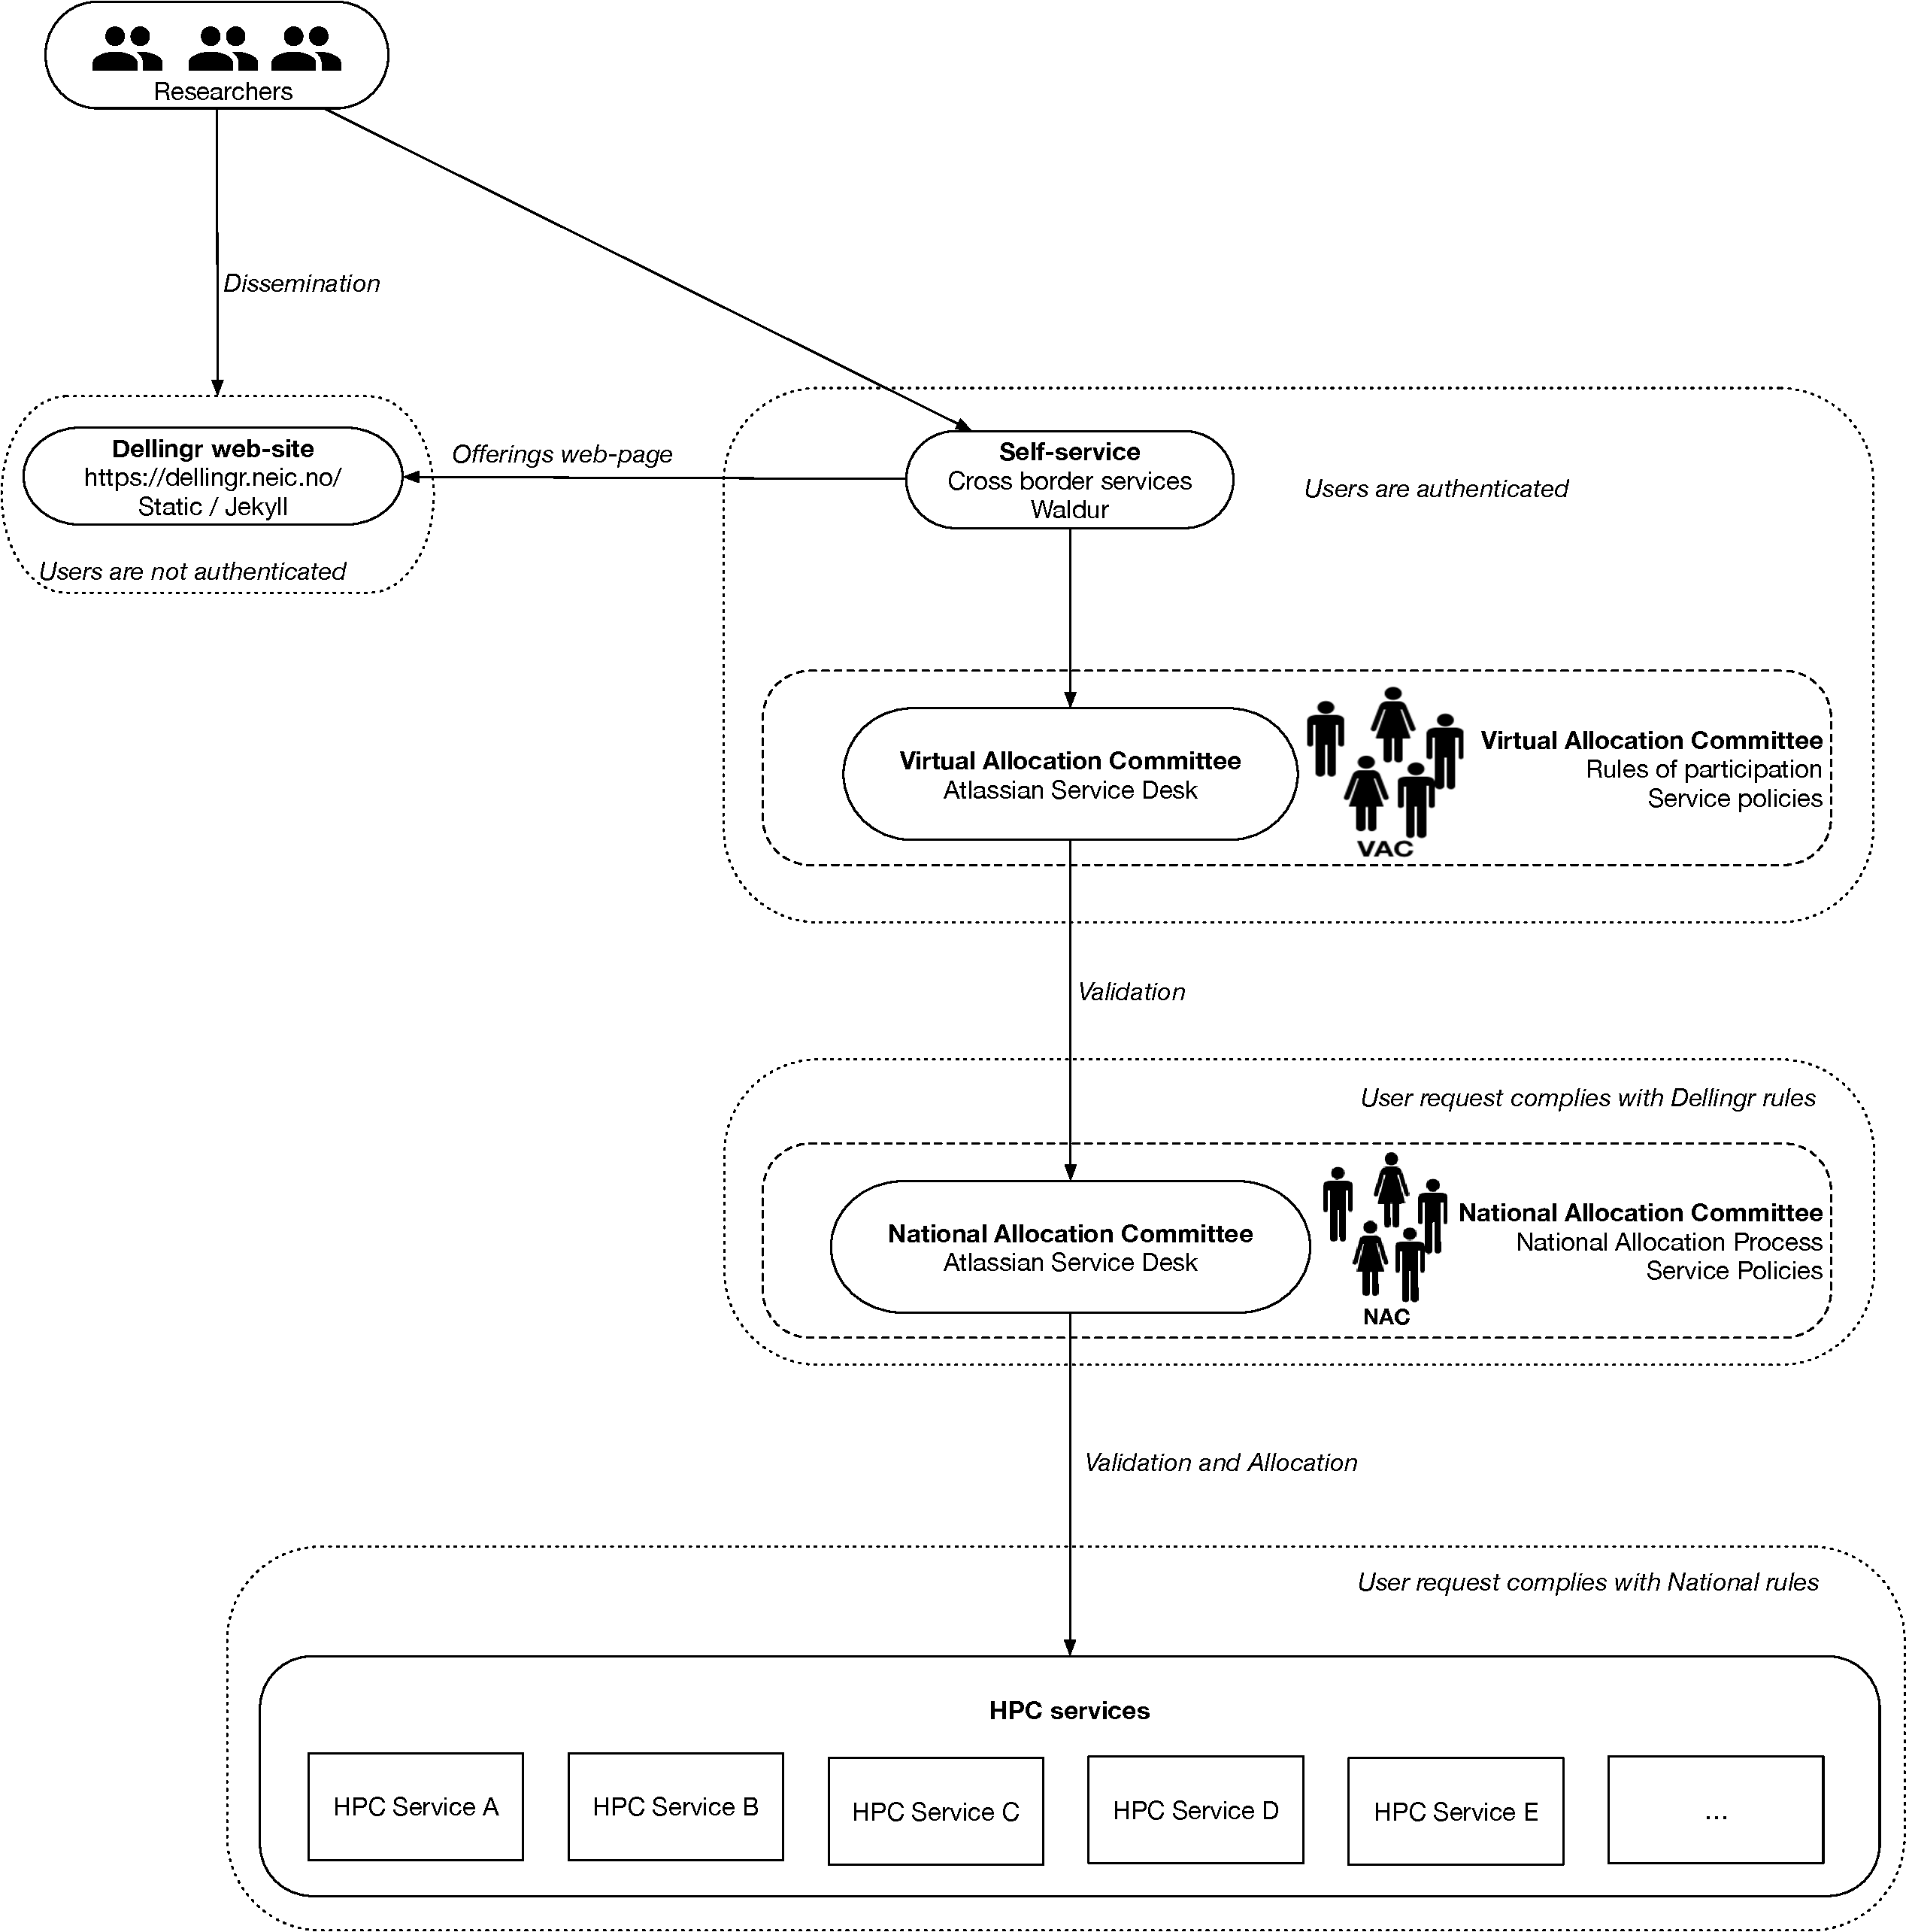
\includegraphics[height=450pt]{diagram.pdf}
\caption{Overview of the second \dell pilot setup}
\end{figure}

First of all, we have adjusted the \dell project website so it can be used as a landing page~\cite{dellingr-landing} for new users willing to get access to resources and used in promotional activities. 
The website is public and does not require any authentication.
The main components of the website included:
\begin{itemize}
    \item Description of rules of participation in the second pilot: \url{https://dellingr.neic.no/apply/}.
    \item Guide for applying for resources via \dell self-service: \url{https://dellingr.neic.no/guide/}.
    \item Up to date list of computational services available to the users along with some basic technical and performance properties: \url{https://dellingr.neic.no/offerings/}.
\end{itemize}
% Once the anonymous user decided that some resources available Dellingr offer is interesting, application process would start. 
Once the user had decided that some \einfra resources available in the \dell offer were interesting, the application process would start. 

\subsection{Application Process}
\label{ssec:application}

As the first step of the application process, a user had to authenticate into the \dell self-service portal using an identity provider from eduGAIN~\cite{edugain}. 
Two results were received through the usage of eduGAIN:
\begin{itemize}
    \item A reliable name and unique ID of the user in the eduGAIN federation;
    \item The domain of the organization that user belongs to.
\end{itemize}
Unfortunately without the authentication service containing reliable information on the group information about the user (affiliation, role), 
the only reliable affiliation information that could be obtained came from the domain attribute in the SAML assertion from eduGAIN. 
This meant that the user had to register their own organization by filling in the form in the self-service portal and that this affiliation information had to be manually confirmed at a later stage.

Once the user has created their organization, they are able to browse resources available for request at that moment in time. 
Over the period of the second pilot, some resources can be activated, archived or paused by the resource owners.
These actions cause the system information to be updated in the self-service portal and the user can see these changes at once.

We initially hoped to be able to automate the whole process of delivery at least for some services, however the amount of issues connected with that was eventually beyond the scope of \dell resources and it was decided to use a service desk system, Jira~\cite{jira}, for processing requests instead. 
Please note that despite this technical limitation, the process is exactly the same for both the manual and automated way.

The user had to also fill in the project information, which has been attached to all requests for resources under that project.
When requesting a resource, users had to:
\begin{itemize}
    \item Provide estimated requirements of resources in terms of CPU and GPU hours;
    \item Provide the science domain (following the standard from~\cite{science-domains}) for which the resources were planned to be used;
    \item Provide nationalities of the users that were expected to get access to the resource.
    \item Agree to the terms of services of the chosen service.
\end{itemize}

Once the user submitted the information, a request to \textbf{Virtual Allocation Committee} (\textbf{VAC}) was been created. 
Upon receiving notification about new requests, the VAC validated input data to see if it complies with the Rules of participation of \dell -- and if so, forwarded the requests to the representative of the service, aka \textbf{National Allocation Committee} (\textbf{NAC}).

NACs took as input request for allocation that had the minimal commonly agreed information (see above) as well as validation of VAC that request confirms to the \dell policy. NAC representative then could decide if the request also matches with requested resource policies and either grant or deny the application. 

To make sure that process works smoothly, a separate role –– service manager –– was in place to follow up on created tickets and assure that requests are processed in time.

\subsection{Resources}

One of the most often asked question was 'What resources do you have'? To make sure that the answer is visible to the widest audience, we have collected various technical information about the services and exposed parts of it on the public website. Exposure was semi-automated, taking the JSON from the self-service (automatic) copying it to the \dell website (manual) and publishing it as static website in Jekyll (automatic). This has allowed to significantly reduce getting authenticated requests from users (which lead to request processing flow), who would not benefit from the provided offerings.  

Over time some service offerings have been taken of the list due to different reasons, an example of state of affairs in the middle of February is shown below. Site properties were selected based on the main questions asked. One of the most requested resources was GPU access, however only one offering was providing that, which has hindered high number of requests from arriving.


\begin{figure}
\centering
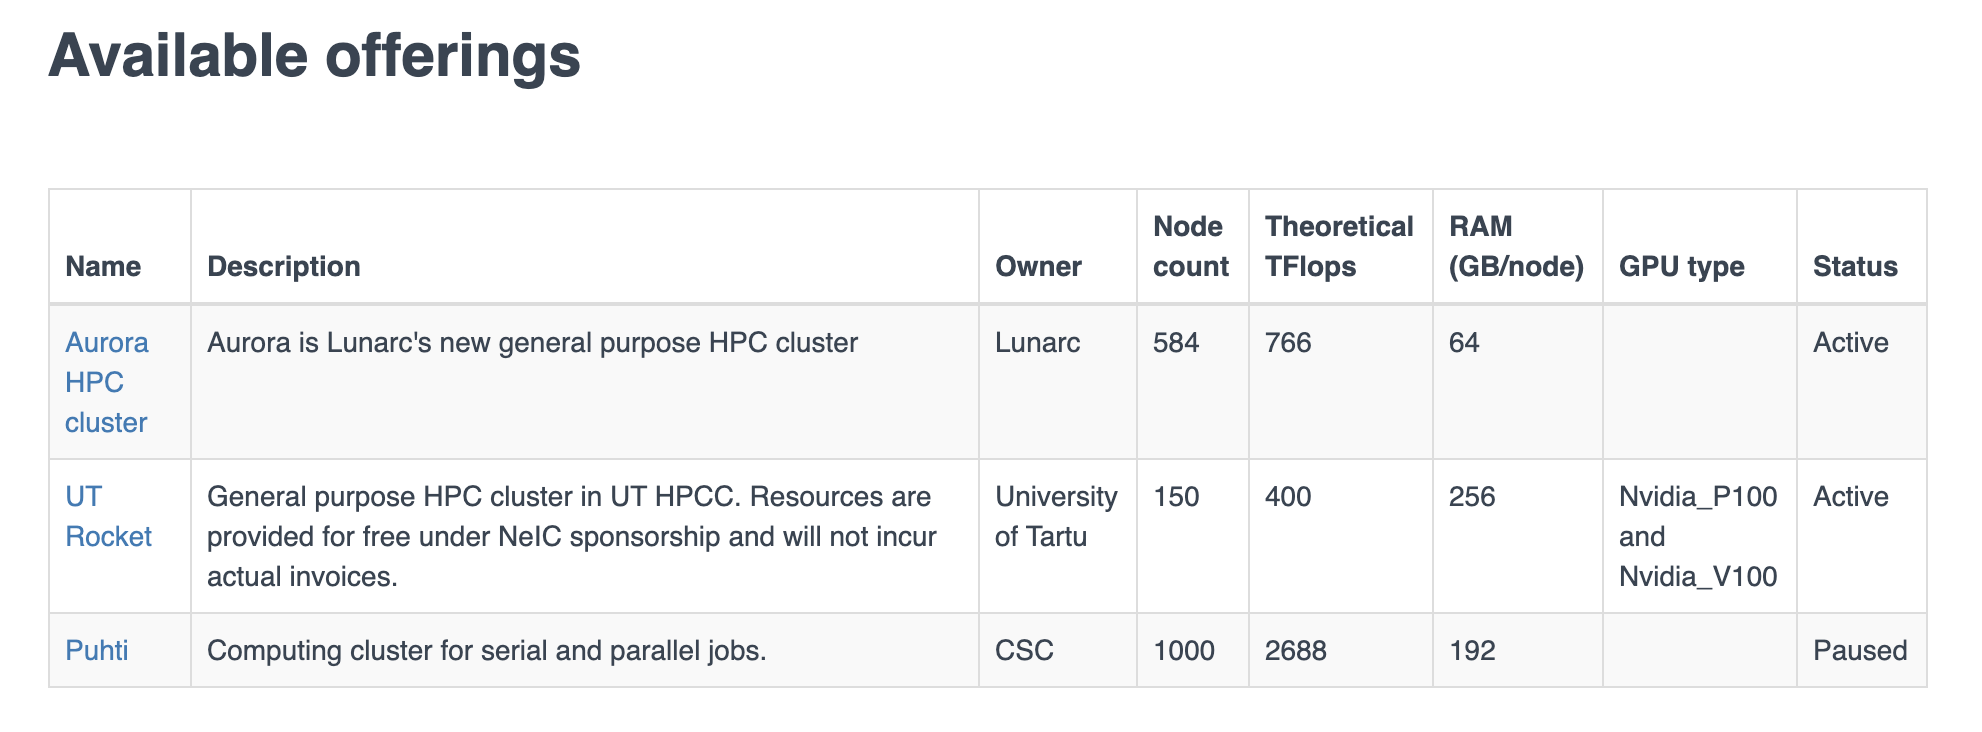
\includegraphics[height=180pt]{Dellingr-list-of-resource.png}
\caption{Example of service offerings shown to users and accessible via the \dell self-service portal.}
\end{figure}

\section{Results}
\label{sec:results}
\newcommand{\BUcons}{6406\xspace}
\newcommand{\BUreq}{134000\xspace}

In this \pilot the resources were allocated in a different manner than the first pilot.
In this case the users requested specific resources not in their country through the portal. 
In the first pilot, the users requested an amount of computing time and were assigned to a resource manually by the \dell project.
Also, the portal expressed the \einfra resources in a common format ``Billing Units" (BU)~\footnote{In general for all \dell resources, 1 CPU core has been set to cost 0.01 BU per month and one GPU core cost is 0.1 BU per month.}.

The \dell \pilot was launched in June~2019 and the last applications were received in December~2019. 
These figures summarize the extent of the Pilot~\footnote{As of \today}:
\begin{itemize}
\item 14 applications were received;
\item 12 projects were accepted;
\item \BUreq BU were granted to the accepted projects;
\item \BUcons BU were consumed by the projects.
\end{itemize}
Only two applications were rejected. 

Table~\ref{tab:projects} shows the orders for resources received from users.
\begin{table}
\begin{center}
\rowcolors{2}{gray!25}{white}
\begin{tabular}{|p{7cm}|l|l|r|r|} \hline
\bf Project Title & \bf From & \bf To &\bf Requested &\bf Used \\
                  & & & {\bf BU} & {\bf BU} \\ \hline
Exploring mechanisms of roughness creation at the nanoscale using a systematic set of large time and length scale Molecular Dynamics simulations. & DK & EST & 500 & {2085}\\

Acetonitrile parametrization. & DK & FI & 50000 & 482.94 \\

Local structural correlations in Sn doped BCZT ferroelectric relaxors & DK & SE & 3000 & 1569\\

GETM high-resolution modelling for the Baltic Sea. & EST & SE & 500 & 594 \\

Simulating Electronic and Nuclear Dynamics in Dye-Sensitized Solar Cells. & FI & EST & 2000 & \\

Fluid reactions mechanism on mineral surface in planet interior. & IS & SE & 2000 & n/a \\

Simulation of ions in solutions using QM/MM method. & IS & FI & 10000 & 3.58 \\

Simulating Electronic and Nuclear Dynamics in Dye-Sensitized Solar Cells & IS & FI & 5000 & 6.99 \\

Benchmark comparison of pure, hybrid, double-hybrid DFT functionals against the highly accurate wavefunction methods for reliability for quantum dynamics simulations. & IS & FI & 5000 & 3.85 \\

Configuration space sampling of solvated hexaaquairon(II) and hexaaquairon(III). & IS & FI & 2000 & 51.30 \\

Polarizable Embedding of Ions in Solution. & IS & FI & 2000 & 0 \\

Atomistic insight into difference and similarities of copper sulfide and oxide corrosion films. & SE & FI & 50000 & 1609.42 \\

\bf Total & & & \BUreq & \BUcons \\\hline
\end{tabular}
\caption{Another convincing explanation.(DK=Denmark, EE=Estonia, FI=Finland, IS=Iceland, NO=Norway, SE=Sweden). \label{tab:projects}}
\end{center}
\end{table}
% \todo[inline]{AS: There was a continuation project of the Danish project from the first pilot. They only applied through the SUPR interface which is why it doesn't show up in Waldur. The title is "Local structural correlations in Sn doped BCZT ferroelectric relaxors" they requested 75kch/month over 4 months i.e. 300kch=3000bu. I'd say that this should count as well even though they didn't go through the portal.} 
% \todo[inline,backgroundcolor=red!25]{JW: Agree. Will add to the table.}
% \todo[inline]{PN: I added another similar case to the table: Project "Simulating Electronic and Nuclear Dynamics in Dye-Sensitized Solar Cells" is a continuation project from the first pilot, applied through CSC Service Desk.}
% \todo[inline]{PN: I updated Total Requested in the table.}
% \todo[inline]{JW: Updated Table 2.}
As can be seen in Table~\ref{tab:projects} the amount of BUs requested varies over two orders of magnitude.
The amount of BUs consumed by the project also varies from very little (zero) to multiples of the original allocation.
One project, with a BU consumption of "n/a" was not correctly assigned an allocation due to a misunderstanding in the project setup stages.

Table~\ref{tab:results} shows the resource requests between client and hosting countries.
\begin{table}[ht]
\begin{center}
% \vspace{0.5cm}
\rowcolors{2}{gray!25}{white}
\begin{tabular}{|l|r|r|r|r|r|r|r|r|} \hline
{\bf Host/Guest} & \bf Denmark & \bf Estonia & \bf Finland & \bf Iceland & \bf Norway$^*$ & \bf Sweden 
& \multicolumn{2}{c|}{\bf Total} \\ \cline{7-9}
 & & & & & & & \multicolumn{1}{r}{\bf BU} & {\bf \#} \\ \hline
\bf Denmark & x & & & & & & 0 & 0\\
\bf Estonia & 500 & x & 2000 & & & & 2500 & 2 \\
\bf Finland & 50000 & & x & 26000 & & 50000 & 126000 & 7 \\
\bf Iceland & & & & x & & & 0 & 0\\
\bf Norway$^*$  & & & & & x & & 0 & 0\\
\bf Sweden  & 3000 & 500 & & 2000 & & x & 5500 & 3 \\
\hline
\bf Total BU (\#) & 53500 (3) & 500 (1) & 2000 (1) & 28000 (6) & 0 & 50000 (1) & \BUreq & 12 \\ \hline
\end{tabular}
\caption{The number of BUs requested and hosted per country. The horizontal (vertical) view gives the number of BUs hosted (requested) per country. $*$ Norway has observer status only.\label{tab:results}}
% \vspace{0.5cm}
\end{center}
\end{table}
As the number of accepted projects was 12 and the number of entries in Table~\ref{tab:results} is 8, it can be seen that most countries managed to generate 1 request.
The exception to this was Iceland that generated 6 projects and, to a lesser extent, Denmark that generated 3 projects.
It can be seen in Table~\ref{tab:results} that one country (Finland) hosted the majority of the projects and BUs and one country (Iceland) generated the 
majority of the projects but not the majority of the BUs requested.


\section{Conclusions}

Overall, we see that the process implemented during the second pilot of \dell is:
\begin{itemize}
\item not very intrusive for the service providers;
\item scalable in the number of participating users and organizations, both consumers and service providers;
\item provided additional benefits beyond the initial scope, e.g. creating a small up-to-date public catalogue of HPC services in the Nordic region without extra effort.
\end{itemize} 

User feedback was requested from the participants who requested and received an allocation of BUs in the pilot.
Of the 12 projects accepted, we received answers from 6 of the users.
The respondents are split evenly between those that had participated in the first pilot and those who had not.
The users generally found it easy to access the ``foreign" \einfra resources, probably due to the refined procedures to accept users developed by the NACs of the national \einfra providers.
In general, these users did not have application or licencing support issues.
This might be because users are requesting through a self-service portal to run on non-local resources and are therefore more likely to have open-source software.
Of the users that have not used their allocated resources~\footnote{As of \today}, all indicated that they intend to do so.
None of the respondent users replied that this type of resource sharing/access
is not useful.
A response from more than one user indicated that this is useful for early stage researchers and method development.
The user feedback, provided in the Appendix below, has been generally favourable, which is both motivating and hints that such service could be sustained beyond the \dell lifetime.

As part of the ``contract" between \dell, NeIC and the pilot participants is that any work resulting from the \einfra resources accessed should have an attribution attached: 
``This work was made possible (in part) by usage of computing resources at (institution) through the NeIC Dellingr resource sharing pilot.''
The publications from the 1$^{\rm st}$ \dell pilot can be seen at~\cite{pilot-pubs}.
Due to the length of time for the process from data analysis to publication, it is not expected to receive notice of publications attributed to this second pilot before the official end of the \dell project.

\newpage
\bibliography{main}{}
\bibliographystyle{unsrt}

\newpage
\begin{appendices}

\section{Responses from Framework users}
\label{app:answers}
{
The responses from the participants of the \pilot are given below.
The identities of the participants are intentionally removed.

\subsection*{Responses 1}
\begin{verbatim}
- If you are a user of both the first and second Dellingr pilots... How
     does the experience compare between the two pilots?

I wasn't. 

- How easy was it to get the account on the "foreign" shared resources?

To be perfectly honest, I found the infrastructure around getting accounts and project management 
etc slightly byzantine. But it probably wasn't helped by the fact that I kinda got stuck with two 
accounts for some reason related to my dual employment at two different universities, both using 
the wayf login. What I'm saying is, it was 50%-75% my own fault :) 

- Did you need application support? If so, did it work well?

No.

- Did you have licensing issues? Were they solved?

No issues

- If your project did not use all the allocated resources, why was this
     the case?

I think I used almost all of them, if not all. 

- Other comments on the application framework and/or process?


None i can think of currently. Thanks for letting me be  part of the pilot!
\end{verbatim}
\subsection*{Responses 2}
\begin{verbatim}
- If you are a user of both the first and second Dellingr pilots... How does the experience
compare 
between the two pilots?

I have been using resources from CSC/Finland in both pilots. The experiences have been rather
similar, in both cases positive throughout. Their are two large differences between the rounds 
are: 
i) the new application system for the latest round, which was a bit tricky to understand at
first but the platform seems to have good future potential; 
ii) the new computer cluster at csc (puhti), which works very well.

- How easy was it to get the account on the "foreign" shared resources?
It was easy the first round, and this time I already had an account making it very smooth.

- Did you need application support? If so, did it work well?
Not this round. Last round we had minor issues that the support could solve quickly

- Did you have licensing issues? Were they solved?
Not this round. Last round we needed to confirm our VASP license, which took a few days. 
This is however very common for this program.

- If your project did not use all the allocated resources, why was this the case?
We have not yet had time to use all, but we will.

- Other comments on the application framework and/or process?
Not at this point, other than that is has been working well and that I consider this a very useful 
and good initiative
\end{verbatim}
\subsection*{Responses 3}
\begin{verbatim}

- If you are a user of both the first and second Dellingr pilots... How does the experience
compare between the two pilots?

I did not participate to the first Dellingr pilot.

- How easy was it to get the account on the "foreign" shared resources?

The process for setting up an account to use the CSC resources was easy.

- Did you need application support? If so, did it work well?

I did not.

- Did you have licensing issues? Were they solved?

I did not have any licensing issues.

- If your project did not use all the allocated resources, why was this the case?

I did not use all of the allocated resources because the development and implementation part of 
my project took longer than what initially expected.

- Other comments on the application framework and/or process?

My Dellingr project on CSC terminates on 29.01.2020. Would it be possible to extend the end 
of the project so I can continue using the allocated resources? Or should this be handled 
by CSC?
\end{verbatim}
\subsection*{Responses 4}
\begin{verbatim}

"If you are a user of both the first and second Dellingr pilots... How does the experience
compare between the two pilots?"

-> I cannot answer this question because I am a user of the second Dellingr pilot project. 

"How easy was it to get the account on the "foreign" shared resources?"

-> It was easy as I got the computational budget within 48 hours. The application form was also
straightforward and did not require many details. 

- Did you need application support? If so, did it work well?

-> I filled in the online form myself. The manual for completing the application is clear. 

- Did you have licensing issues? Were they solved?

-> No, I do not. 

- If your project did not use all the allocated resources, why was this the case?

-> This case did not apply to me as I just got the resources a month ago. 

- Other comments on the application framework and/or process?

-> Please continue the project as it is really helpful for early-stage researcher. 
\end{verbatim}
\subsection*{Responses 5}
\begin{verbatim}

- If you are a user of both the first and second Dellingr pilots... How does the experience
compare between the two pilots?

We had positive experience with both pilots. It took us some time in the first pilot to setup
things, but afterward everything was very smooth. For the second pilot, it didn't work
initially because of some misunderstanding (it was not clear on the other side if we got the
approval for the second pilot), but it is working now!

- How easy was it to get the account on the "foreign" shared resources?

Since it was the first time from our university (Aarhus University), it took us some time to
create an account and to make it work. But we did not had any problem afterward.

- Did you need application support? If so, did it work well?

Not that much as we only used LAMMPS software which is straightforward to install. 

- Did you have licensing issues? Were they solved?

No as we only used open-source software

- If your project did not use all the allocated resources, why was this
   the case?

I believe we used even more than allocated resources

- Other comments on the application framework and/or process?

It would be nice to hear about future perspectives of the project and how one can access 
these resources. As I mentioned before, it really helped us a lot.
\end{verbatim}

\subsection*{Responses 6}
\begin{verbatim}
- If you are a user of both the first and second Dellingr pilots. How does the experience 
compare between the two pilots?

The dashboard introduced during pilot phase two was a great boon. Applying for, and monitoring resources, 
was more streamlined.
Pilot phase one was however quite easy to apply for and use.

- Did you need application support? If so, did it work well?

Yes, there was some support needed during pilot phase one,
which was resolved quickly.

- Did you have licensing issues? Were they solved?

No licensing issues. All software used was GNU GPL.

- If your project did not use all the allocated resources, why was this the case?

We still have access to and are using resources from pilot phase two.
Resources from pilot phase one were used fully.

- Other comments on the application framework and/or process?

Keep up the good work. Having an option of applying for computational resources through a shared network 
like this is invaluable for method development.
\end{verbatim}
}


\newpage
\section{Author Information}
\label{app:authors}
\begin{tabular}{lll}
{\bf Name} & {\bf email address} & {\bf ORCID} \\
% Anna Jonna {\'A}rmannsd{\'o}ttir & {\tt annaj@hi.is} & 
Mathias Br{\"a}nnvall & {\tt mathias.brannvall@it.uu.se}; & 0000-0003-4979-4123 \\
Juha Fagerholm & {\tt juha.fagerholm@csc.fi} & 0000-0002-9972-4468 \\
Jens Svalgaard Kohrt & {\tt svalgaard@sdu.dk} & 0000-0002-3104-0406 \\
Ivar Koppel & {\tt ivar.koppel@ut.ee} &  \\
% Bj{\o}rn Lindi & {\tt bjorn.lindi@ntnu.no} &  \\
Ilja Livenson & {\tt ilja.livenson@ut.ee} & 0000-0002-4011-8367 \\
Petri Nikunen & {\tt petri.nikunen@csc.fi} & 0000-0003-0759-6372 \\
Ahti Saar & {\tt Ahti.Saar@ut.ee} & 0000-0003-0642-961X \\
Anders Sj{\"o}str{\"o}m & {\tt Anders.Sjostrom@lunarc.lu.se} & 0000-0003-2213-2138 \\
Hj{\"o}rleifur Sveinbj{\"o}rnsson & {\tt hs@hi.is} &  0000-0002-4120-1234 \\
%% M{\'a}ni Mar{\'i}us Vi{\dh}arsson & {\tt mani@hi.is} &  \\
John White & {\tt john.white@cern.ch} & 0000-0001-5614-0895 \\
\end{tabular}


\end{appendices}

\end{document}
